\newpage

% =========================================================
% ВАРИАНТ 19
% =========================================================

\section*{Вариант 19}

Найдите площадь прямоугольного треугольника, если его катет
и гипотенуза равны соответственно \(15\) и \(17\).

\begin{center}
\begin{tikzpicture}[
  scale=1.1,
  line cap=round,
  line join=round,
  every node/.style={font=\small}
]
  % Треугольник со сторонами 8, 15 и 17
  \coordinate (C) at (0,0);
  \coordinate (A) at (0,3.75);
  \coordinate (B) at (2,0);

  \draw[line width=0.9pt]
    (A)--(B)--(C)--cycle;

  \pic[
    draw,
    line width=0.65pt,
    angle radius=3.2mm
  ] {right angle=A--C--B};

  \path (A)--(C)
    node[midway,left=2mm] {$15$};

  \path (A)--(B)
    node[midway,above right] {$17$};

  \node[above]       at (A) {$A$};
  \node[below right] at (B) {$B$};
  \node[below left]  at (C) {$C$};
\end{tikzpicture}
\end{center}

\[
\boxed{\text{Ответ: }60}
\]


% =========================================================
% ВАРИАНТ 20
% =========================================================

\section*{Вариант 20}

В треугольнике \(ABC\) средняя линия \(DE\) параллельна стороне \(AB\).
Найдите площадь треугольника \(ABC\), если площадь трапеции \(ABED\)
равна \(48\).

\begin{center}
\begin{tikzpicture}[
  scale=0.95,
  line cap=round,
  line join=round,
  every node/.style={font=\small}
]
  \coordinate (A) at (0,0);
  \coordinate (B) at (6,0);
  \coordinate (C) at (4.2,4.4);

  % Середины сторон AC и BC
  \coordinate (D) at ($(A)!0.5!(C)$);
  \coordinate (E) at ($(B)!0.5!(C)$);

  \draw[line width=0.9pt]
    (A)--(B)--(C)--cycle;

  \draw[line width=0.9pt]
    (D)--(E);

  \node[below left]  at (A) {$A$};
  \node[below right] at (B) {$B$};
  \node[above]       at (C) {$C$};
  \node[left]        at (D) {$D$};
  \node[right]       at (E) {$E$};

  \node at (3.15,1.15) {$S_{ABED}=48$};
\end{tikzpicture}
\end{center}

\[
\boxed{\text{Ответ: }64}
\]


% =========================================================
% ВАРИАНТ 21
% =========================================================

\newpage

\section*{Вариант 21}

Периметр прямоугольной трапеции, описанной около окружности, равен \(100\),
её большая боковая сторона равна \(37\).
Найдите радиус окружности.

\begin{center}
\begin{tikzpicture}[
  line cap=round,
  line join=round,
  every node/.style={font=\small}
]
  % Высота трапеции равна 13, поэтому радиус равен 6,5.
  % Основания выбраны так, чтобы большая боковая сторона была равна 37.
  \pgfmathsetmacro{\s}{0.13}
  \pgfmathsetmacro{\h}{13*\s}
  \pgfmathsetmacro{\r}{6.5*\s}
  \pgfmathsetmacro{\a}{(25+10*sqrt(3))*\s}
  \pgfmathsetmacro{\b}{(25-10*sqrt(3))*\s}

  \coordinate (A) at (0,0);
  \coordinate (B) at (\a,0);
  \coordinate (C) at (\b,\h);
  \coordinate (D) at (0,\h);
  \coordinate (O) at (\r,\r);

  \draw[line width=0.9pt]
    (A)--(B)--(C)--(D)--cycle;

  \draw[line width=0.9pt]
    (O) circle (\r);

  \pic[
    draw,
    line width=0.6pt,
    angle radius=3mm
  ] {right angle=D--A--B};

  \pic[
    draw,
    line width=0.6pt,
    angle radius=3mm
  ] {right angle=A--D--C};

  \path (B)--(C)
    node[midway,above right] {$37$};

  \node at (2.8,0.65) {$P=100$};

  \node[below left]  at (A) {$A$};
  \node[below right] at (B) {$B$};
  \node[above right] at (C) {$C$};
  \node[above left]  at (D) {$D$};
\end{tikzpicture}
\end{center}

\[
\boxed{\text{Ответ: }6{,}5}
\]


% =========================================================
% ВАРИАНТ 22
% =========================================================

\section*{Вариант 22}

В четырёхугольник \(ABCD\) вписана окружность,
\(AB=8\), \(BC=5\), \(CD=27\).
Найдите четвёртую сторону четырёхугольника.

\begin{center}
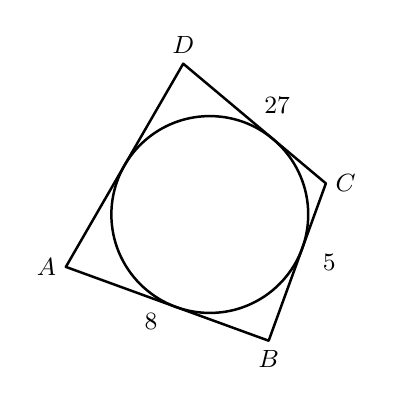
\begin{tikzpicture}[
  scale=1.25,
  line cap=round,
  line join=round,
  every node/.style={font=\small}
]
  \coordinate (O) at (0,0);

  % Четырёхугольник, описанный около единичной окружности
  \coordinate (A) at (-1.462,-0.532);
  \coordinate (B) at ( 0.598,-1.282);
  \coordinate (C) at ( 1.179, 0.316);
  \coordinate (D) at (-0.270, 1.532);

  \draw[line width=0.9pt]
    (A)--(B)--(C)--(D)--cycle;

  \draw[line width=0.9pt]
    (O) circle (1);

  \path (A)--(B)
    node[midway,below left] {$8$};

  \path (B)--(C)
    node[midway,right=2mm] {$5$};

  \path (C)--(D)
    node[midway,above right] {$27$};

  \node[left]  at (A) {$A$};
  \node[below] at (B) {$B$};
  \node[right] at (C) {$C$};
  \node[above] at (D) {$D$};
\end{tikzpicture}
\end{center}

\[
\boxed{\text{Ответ: }30}
\]


% =========================================================
% ВАРИАНТ 23
% =========================================================

\newpage

\section*{Вариант 23}

Площадь параллелограмма \(ABCD\) равна \(145\).
Найдите площадь параллелограмма \(A'B'C'D'\),
вершинами которого являются середины сторон данного параллелограмма.

\begin{center}
\begin{tikzpicture}[
  scale=0.9,
  line cap=round,
  line join=round,
  every node/.style={font=\small}
]
  \coordinate (A) at (0,0);
  \coordinate (B) at (5.6,0);
  \coordinate (D) at (1.2,3.1);
  \coordinate (C) at (6.8,3.1);

  % Середины сторон параллелограмма
  \coordinate (Ap) at ($(A)!0.5!(B)$);
  \coordinate (Bp) at ($(B)!0.5!(C)$);
  \coordinate (Cp) at ($(C)!0.5!(D)$);
  \coordinate (Dp) at ($(D)!0.5!(A)$);

  \draw[line width=0.9pt]
    (A)--(B)--(C)--(D)--cycle;

  \draw[line width=0.9pt]
    (Ap)--(Bp)--(Cp)--(Dp)--cycle;

  \fill (Ap) circle (1.1pt);
  \fill (Bp) circle (1.1pt);
  \fill (Cp) circle (1.1pt);
  \fill (Dp) circle (1.1pt);

  \node[below left]  at (A) {$A$};
  \node[below right] at (B) {$B$};
  \node[above right] at (C) {$C$};
  \node[above left]  at (D) {$D$};

  \node[below] at (Ap) {$A'$};
  \node[right] at (Bp) {$B'$};
  \node[above] at (Cp) {$C'$};
  \node[left]  at (Dp) {$D'$};

  \node at (3.4,1.55) {$S_{ABCD}=145$};
\end{tikzpicture}
\end{center}

\[
\boxed{\text{Ответ: }72{,}5}
\]


% =========================================================
% ВАРИАНТ 24
% =========================================================

\section*{Вариант 24}

Два угла вписанного в окружность четырёхугольника равны
\(112^\circ\) и \(125^\circ\).
Найдите больший из оставшихся углов.
Ответ дайте в градусах.

\begin{center}
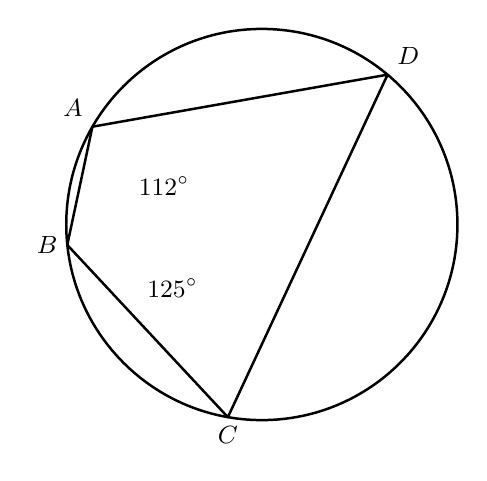
\begin{tikzpicture}[
  scale=1.08,
  line cap=round,
  line join=round,
  every node/.style={font=\small}
]
  \def\R{2.3}

  \coordinate (O) at (0,0);

  % Координаты обеспечивают углы A=112 градусов и B=125 градусов
  \coordinate (A) at (150:\R);
  \coordinate (B) at (186:\R);
  \coordinate (C) at (260:\R);
  \coordinate (D) at (50:\R);

  \draw[line width=0.9pt]
    (O) circle (\R);

  \draw[line width=0.9pt]
    (A)--(B)--(C)--(D)--cycle;

  \node at (-1.15,0.45) {$112^\circ$};
  \node at (-1.05,-0.75) {$125^\circ$};

  \node[above left]  at (A) {$A$};
  \node[left]        at (B) {$B$};
  \node[below]       at (C) {$C$};
  \node[above right] at (D) {$D$};
\end{tikzpicture}
\end{center}

\[
\boxed{\text{Ответ: }68}
\]

\end{document}